% Created 2023-10-04 mié 21:34
% Intended LaTeX compiler: pdflatex
\documentclass[11pt]{article}
\usepackage[utf8]{inputenc}
\usepackage[T1]{fontenc}
\usepackage{graphicx}
\usepackage{grffile}
\usepackage{longtable}
\usepackage{wrapfig}
\usepackage{rotating}
\usepackage[normalem]{ulem}
\usepackage{amsmath}
\usepackage{textcomp}
\usepackage{amssymb}
\usepackage{capt-of}
\usepackage{hyperref}
\usepackage{../modern}
\bibliography{./fuentes.bib}
\raggedbottom
\setcounter{secnumdepth}{2}
\author{Luis Eduardo Galindo Amaya (1274895)}
\date{4 de Octubre 2023}
\title{Taller 4. Redireccionamiento}
\hypersetup{
 pdfauthor={Luis Eduardo Galindo Amaya (1274895)},
 pdftitle={Taller 4. Redireccionamiento},
 pdfkeywords={},
 pdfsubject={},
 pdfcreator={Emacs 27.1 (Org mode 9.3)}, 
 pdflang={Spanish}}
\begin{document}

\modentitlepage{../images/escudo-uabc-2022-color-cont.png}
\tableofcontents \pagebreak
\datasection{Individual}

\section{Introducción}
\label{sec:org2520a24}
Durante esta practica aprenderemos como utilizar el redireccionamiento en Unix, El redireccionamiento consiste en una capacidad que permite mover datos fácilmente hacia dentro/fuera de los archivos. Usualmente los programas en unix redireccionan su flujo a stdout pero a lo largo de este taller aprenderemos como cambiarlo y utilizarlo para extender las capacidades del sistema.

\pagebreak

\section{Actividades}
\label{sec:org8b0345e}
\subsection{Muestre el archivo billboard con las líneas numeradas}
\label{sec:orgc41ce2a}
\begin{verbatim}
cat -n billboard
\end{verbatim}

\begin{figure}[htbp]
\centering
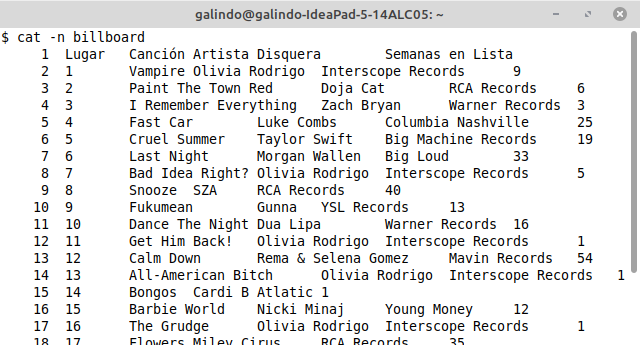
\includegraphics[width=10cm]{img/1.png}
\caption[\texttt{cat -n billboard}]{salida de \texttt{cat -n billboard}}
\end{figure}

\subsection{Muestre solamente a los artistas que pertenecen a RCA Records}
\label{sec:org8e13ac3}
\begin{verbatim}
grep "RCA Records" billboard
\end{verbatim}

\begin{figure}[htbp]
\centering
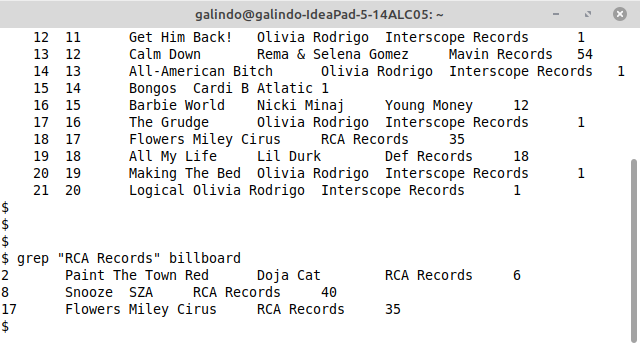
\includegraphics[width=10cm]{img/2.png}
\caption[\texttt{grep}]{\texttt{grep} sin argumentos nos permite encontrar un texto en un flujo}
\end{figure}

\pagebreak

\subsection{Repita el paso anterior pero ahora redireccione la salida para generar un archivo llamado RCA}
\label{sec:orgbe7fde3}

\begin{verbatim}
grep "RCA Records" billboard > RCA
\end{verbatim}

\begin{figure}[htbp]
\centering
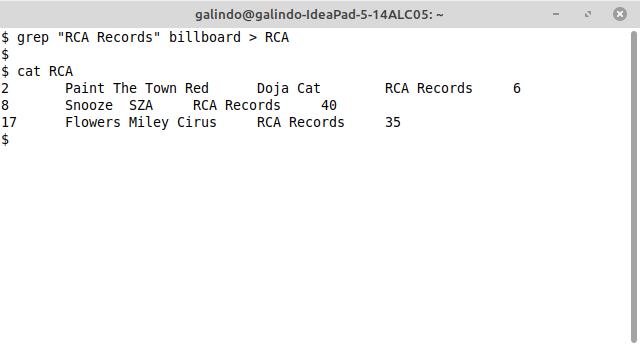
\includegraphics[width=10cm]{img/3.png}
\caption[\texttt{>}]{el caracter \texttt{>} permite redirigir el flujo a otra salida}
\end{figure}


\subsection{Muestre y genere un archivo con los artistas que graban con Warner}
\label{sec:org403140e}
\begin{verbatim}
grep "Warner Records" billboard > Warner
\end{verbatim}

\begin{figure}[htbp]
\centering
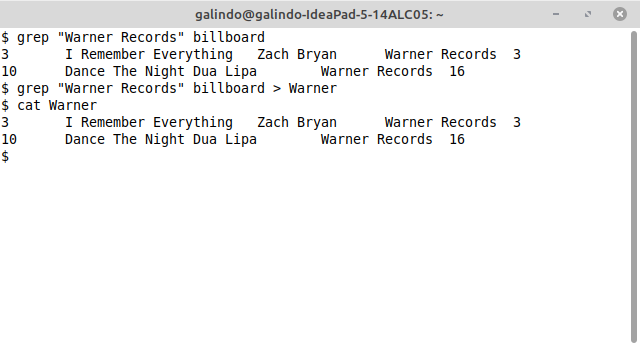
\includegraphics[width=10cm]{img/4.png}
\caption[\texttt{grep "Warner Records" billboard > Warner}]{salida de \texttt{grep "Warner Records" billboard > Warner}}
\end{figure}

\pagebreak

\subsection{Repita el paso anterior pero ahora debe verse en pantalla el resultado al mismo tiempo que se genera el archivo}
\label{sec:orgb5cc61c}

\begin{verbatim}
grep "Warner Records" billboard | tee Warner
\end{verbatim}

\begin{figure}[htbp]
\centering
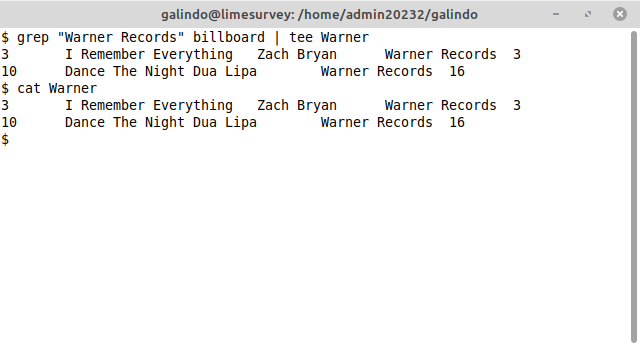
\includegraphics[width=10cm]{img/5.png}
\caption[\texttt{tee}]{El comando \texttt{tee} nos permite ver la salida del comando y escribir en el archivo}
\end{figure}

\subsection{Genere un archivo con las últimas tres líneas del archivo billboard}
\label{sec:org93dd30a}
\begin{verbatim}
tail -n 3 billboard > tres_lineas.txt
\end{verbatim}

\begin{figure}[htbp]
\centering
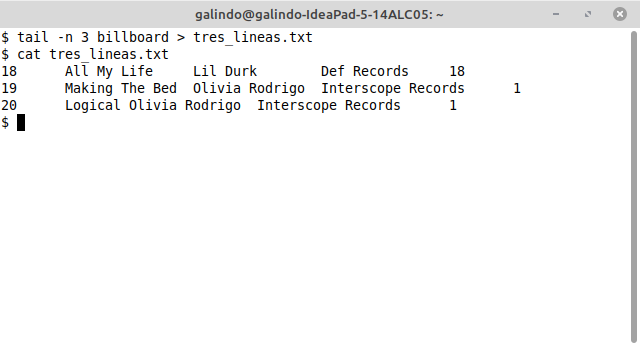
\includegraphics[width=10cm]{img/6.png}
\caption[\texttt{tail -n 3 billboard}]{salida de \texttt{tail -n 3 billboard}}
\end{figure}

\pagebreak

\subsection{Genere un archivo nuevo con el contenido billboard debe estar escrito todo en mayúsculas}
\label{sec:org2db5c79}
\begin{verbatim}
tr '[:lower:]' '[:upper:]' < billboard > bmayusculas.txt
\end{verbatim}

\begin{figure}[htbp]
\centering
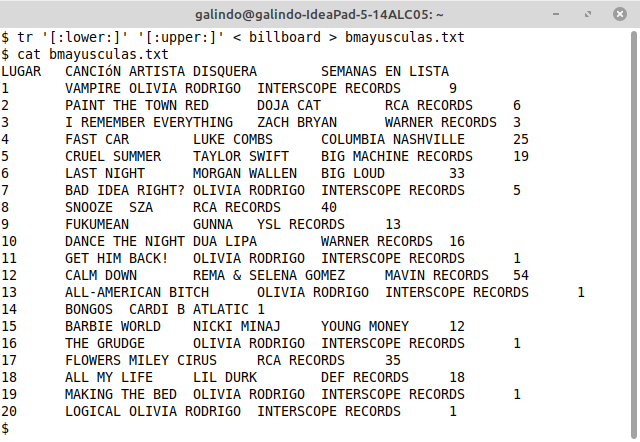
\includegraphics[width=10cm]{img/7.png}
\caption{Reemplazar minúsculas con mayúsculas}
\end{figure}

\subsection{Cree el archivo nombres con solo el primer nombre de las personas aprobadas en lista2023}
\label{sec:orgddb45af}
\begin{verbatim}
grep -v "ORDINARIO" lista2023 | cut -d':' -f3 | tee nombresap.txt
\end{verbatim}

\begin{figure}[htbp]
\centering
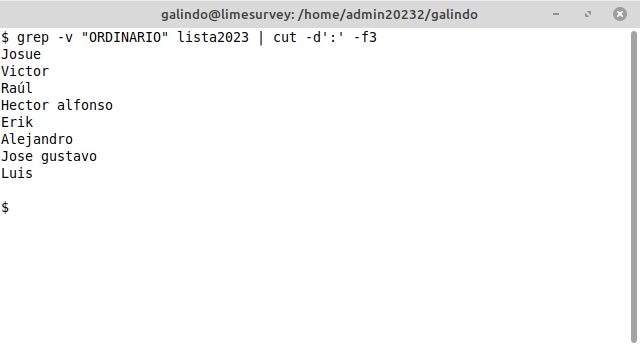
\includegraphics[width=10cm]{img/a8.png}
\caption{nombresap.txt}
\end{figure}


\begin{description}
\item[{grep -v 'ORDINARIO' lista2023}] Se busca todos los elementos que no tengan 'ORDINARIO'
\item[{cut -d':' -f3}] Se obtiene la tercera columna
\item[{tee nombresap.txt}] se muestra en STDOUT y se guarda en un archivo
\end{description}

\pagebreak

\subsection{En el archivo de lista2023 sustituya todos los ':' por espacios}
\label{sec:org30b8bad}
\begin{verbatim}
cat lista2023 | tr ':' ' '
\end{verbatim}

\begin{figure}[htbp]
\centering
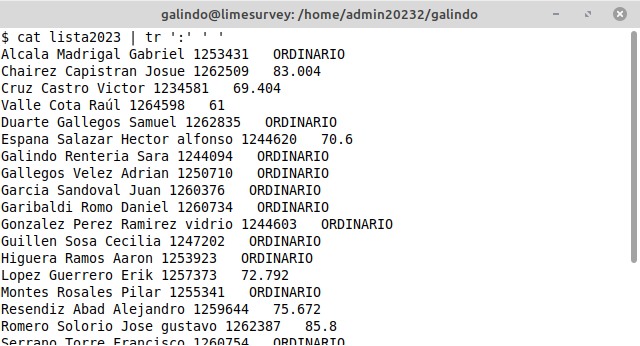
\includegraphics[width=10cm]{img/8.png}
\caption[\texttt{cat lista2023 | tr ':' ' '}]{salida de \texttt{cat lista2023 | tr ':' ' '}}
\end{figure}

\subsection{Genere un archivo que contenga solamente las matriculas de los alumnos aprobados en el archivo lista2023}
\label{sec:org4f944b3}
\begin{verbatim}
grep -v "ORDINARIO" lista2023 > aprobados.txt
cat aprobados.txt
\end{verbatim}

\begin{figure}[htbp]
\centering
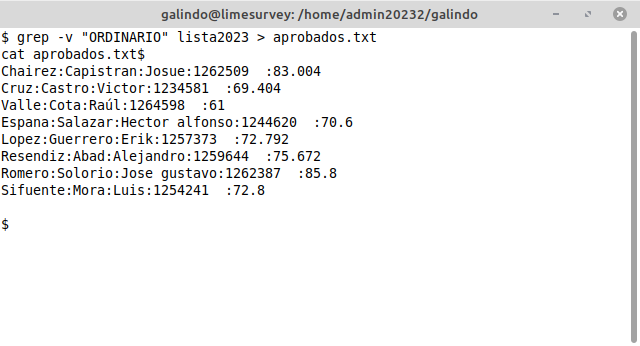
\includegraphics[width=10cm]{img/9.png}
\caption{mostrar el contenido de aprobados.txt}
\end{figure}

\pagebreak

\subsection{En el archivo lista sustituya todas las matriculas por algun otro carácter}
\label{sec:org37a46f0}

\begin{verbatim}
tr "[0-9]" "A" < lista2023
\end{verbatim}

\begin{figure}[htbp]
\centering
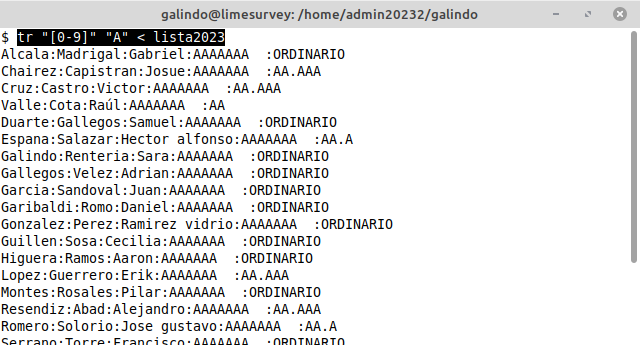
\includegraphics[width=10cm]{img/10.png}
\caption[\texttt{tr '[0-9]' 'A'}]{\texttt{tr '[0-9]' 'A'} Indica todos los caracteres del 0-9 se reemplazaran por 'A'}
\end{figure}

\subsection{Sustituya todos los simbolos de puntuacion en diario por otro carácter}
\label{sec:org723e1e9}

\begin{verbatim}
tr '[:punct:]' 'X' < patria
\end{verbatim}

\begin{figure}[htbp]
\centering
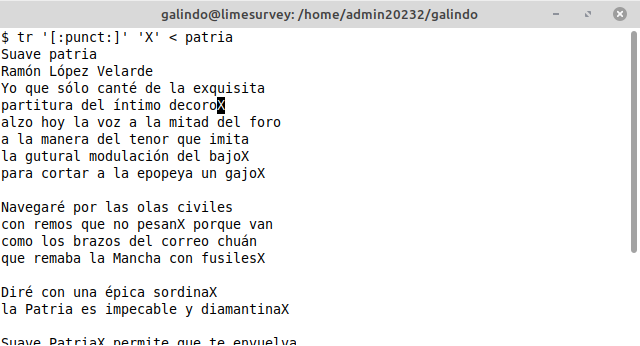
\includegraphics[width=10cm]{img/11.png}
\caption{se reemplazan los puntos y comas por 'X'}
\end{figure}

\pagebreak

\subsection{Genere un archivo solo con las IPs de las personas que están trabajando en el sistema actualmente, pero la salida debe de verse en pantalla al mismo tiempo que se genera el archivo}
\label{sec:orgbf3f52d}
\begin{verbatim}
who | tr -s ' ' | cut -d' ' -f6 | tee ips.txt
\end{verbatim}

\begin{figure}[htbp]
\centering
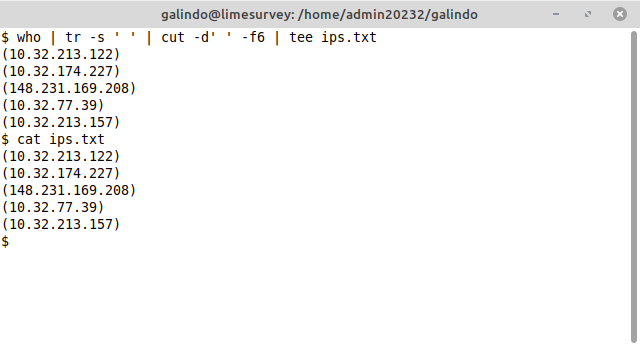
\includegraphics[width=10cm]{img/13.png}
\caption{IPs obtenidas}
\end{figure} 

\begin{description}
\item[{who          }] Muetra quien esta conectado al servidor.
\item[{tr -s ' '    }] Elimina todos los espacio blancos consecutivos\footnote{\cite{StackExchange}}.
\item[{cut -d' ' -f6}] Extrae la 6ta. columns de \texttt{who} (el ip).
\item[{tee ips.txt  }] manda el resultado a stdout y a ips.txt.
\end{description}

\pagebreak

\subsection{Genere un archivo que contenga las lista de usuarios del sistema que pertenecen al mismo grupo que usted,  esten o no actualmente en el sistema}
\label{sec:org5950083}
\begin{verbatim}
cat /etc/passwd | grep "admin20232"
\end{verbatim}

\begin{figure}[htbp]
\centering
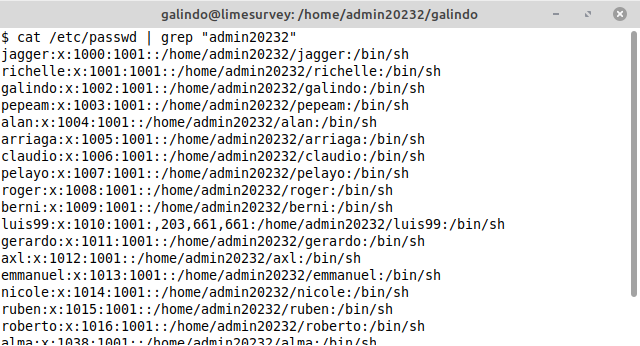
\includegraphics[width=10cm]{img/14.png}
\caption{Miembros de admin20232}
\end{figure}


\cite{A2022}

\subsection{Genere un archivo que contenga el user name y grupo de los usuarios cuyo login name empieza con al}
\label{sec:org05ea107}
\begin{verbatim}
cat /etc/passwd | grep "admin20232" | grep "^al"
\end{verbatim}

\begin{figure}[htbp]
\centering
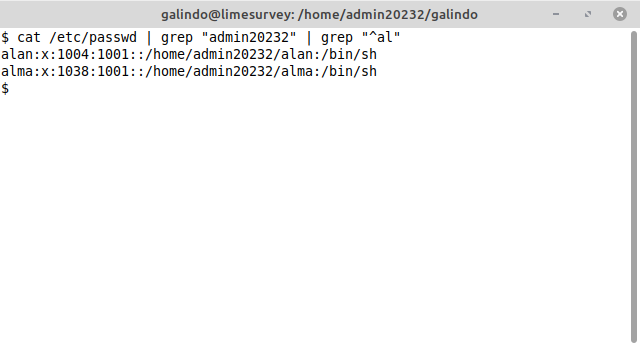
\includegraphics[width=10cm]{img/15.png}
\caption[\texttt{grep '\textasciicircum{}al'}]{\texttt{grep '\textasciicircum{}al'} usa una expresión regular que busca strings que comienzan con al}
\end{figure}


\section{Conclusión}
\label{sec:orgf3993e3}
A lo largo de esta practica aprendí como direccionar flujos de salida con la 
terminal en Linux, anteriormente ya habíamos usado un poco de direccionamiento
por ejemplo al usar el comando \texttt{more} pero en esta practica lo utilizamos ya no 
solamente para mostrar resultados, si no que también como un paso intermedio para
lograr un resultado.

\section{Referencias}
\label{sec:org7008125}
\printbibliography[heading=none]
\end{document}
